
\section{System overview}\label{sec:res:sys}

Some changes are made to Comordo's original system design, as given in \sectionref{sec:task}. The final system is shown in \figureref{fig:sysfinal}.

The logic of the recommender system is built of two major parts: the \textit{reader module} and the \textit{recommender module}. Several modules from the original sketch has become submodules inside the recommender module. This is a logical grouping as the reader module and the recommender module are both implemented as separate scripts and the submodules represents a higher level description of the implemented functionality. 

The \textit{exporter module} is an utility module which generates recommendations from the database into another output format and serves statistics and as a developer debugging tool.  The remote API and the admin web interface are included in the system sketch, but they are not implemented by this thesis.

\begin{figure}[h!]
  \centering
    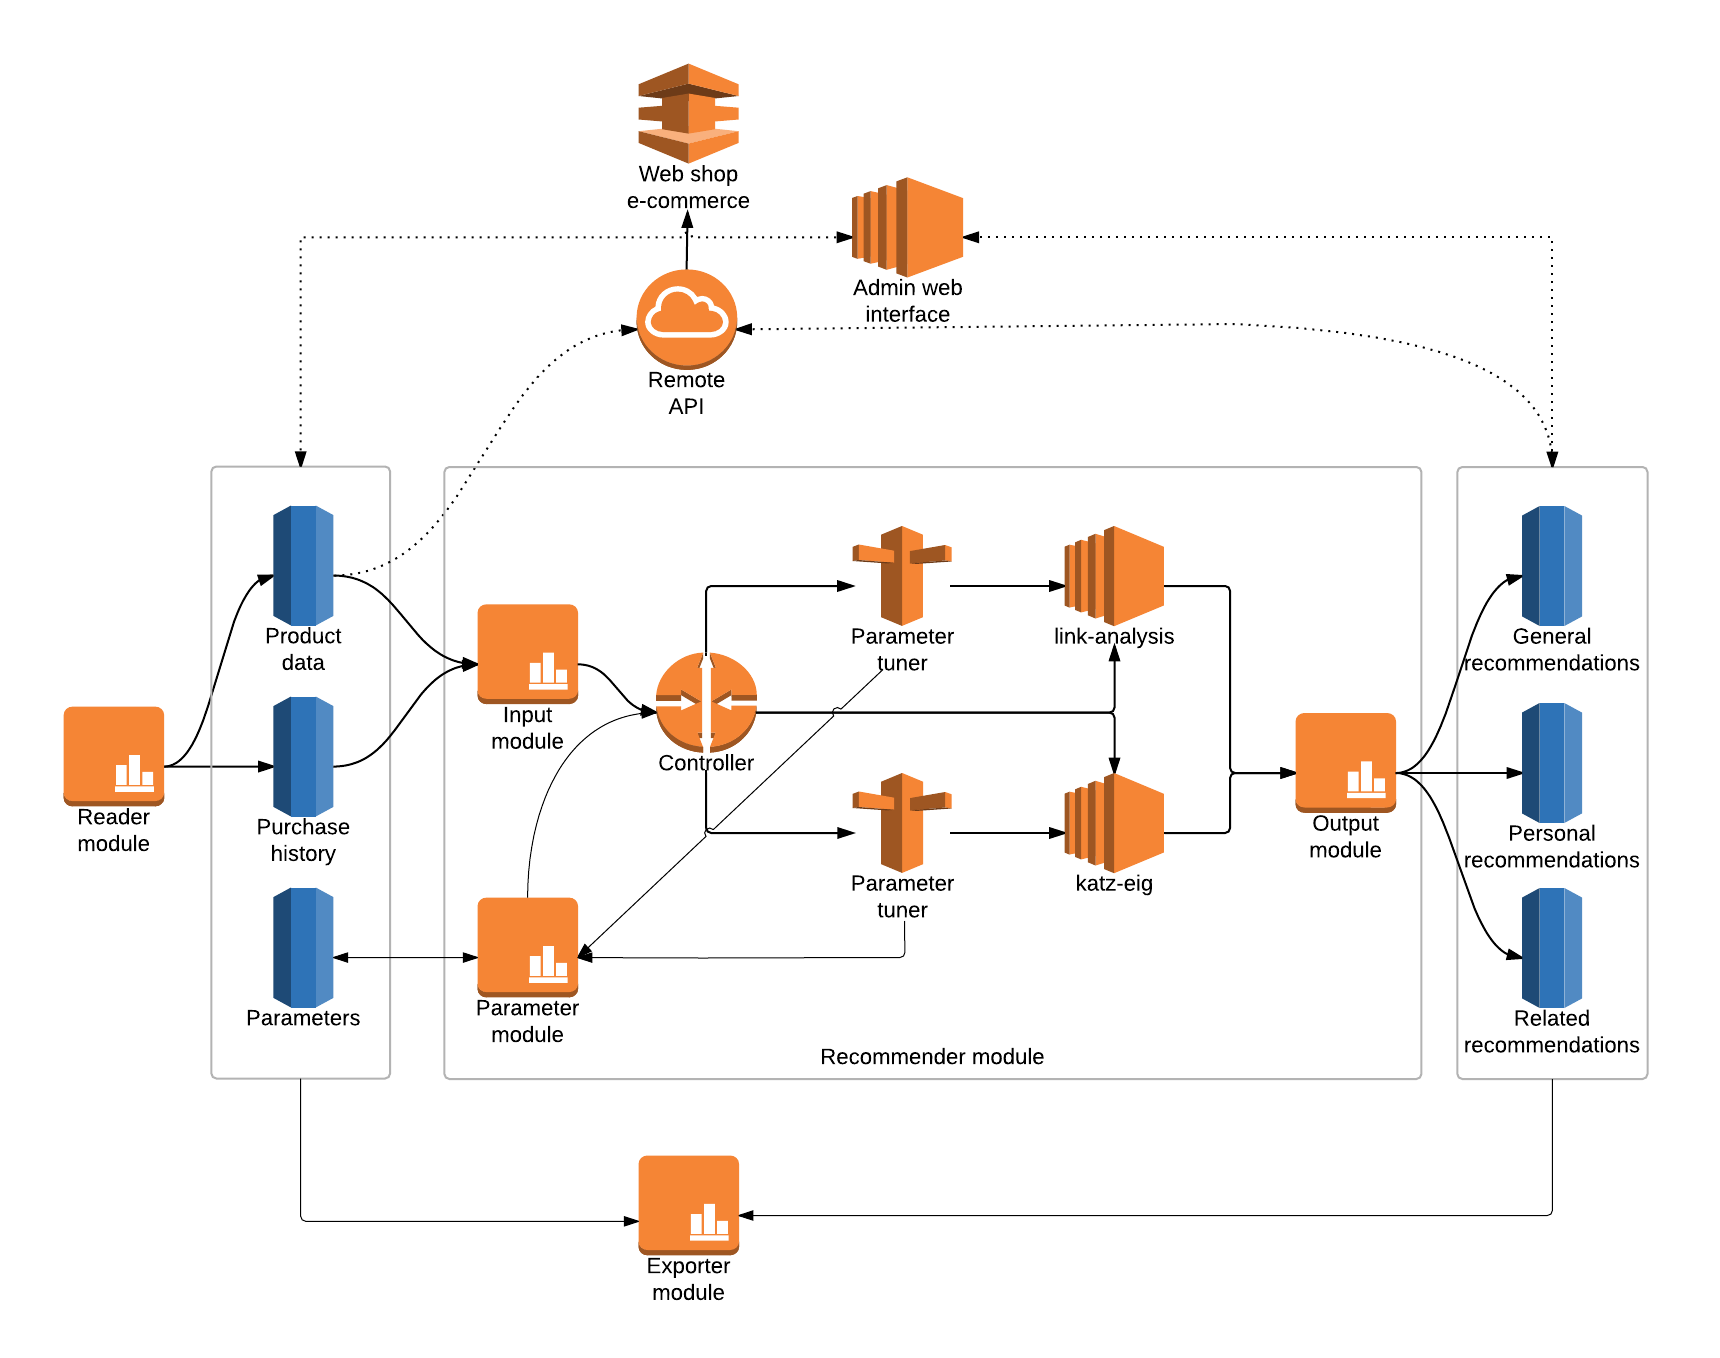
\includegraphics[width=1.0\textwidth]{fig/system_overview_final.png}
  \caption{Overview of the recommender system. Dotted lines represents interactions not implemented by the thesis and the thick lines depicts the flow of generating recommendations.}
  \label{fig:sysfinal}
\end{figure}

\FloatBarrier


\subsection{Reader module}

The reader module takes data files, with client specific formatting, and stores the data in the databases. The data contains user interaction history of some sort, possibly as a list of user-item pairs, but it can also contain additional user and item information all in a single file or in several.

To allow for flexibility the reader module uses a plugin system which can be selected at runtime. This is accomplished using python's dynamic module loading capabilities.

Firstly the reader module will get a list of available plugins found in

\begin{lstlisting}
    lib/reader_plugins
\end{lstlisting}

The plugin class shall have a single uppercase letter and the rest lowercase and reside in a file with all lowercase. For example a plugin which handles \textit{eswc} data could have the class ``Eswc'' inside a file ``eswc.py'' in the plugin directory.

Secondly the appropriate plugin will be selected via command line arguments and the plugin class will be handed control. The class should have two methods: ``add\_arguments'' which parses extra command line arguments and ``load'' which shall return a user hash and a product hash. \Appendixref{sec:eswc_plugin} describes a full example plugin which handles \textit{eswc} data.

With the selected data the reader module can then generate Matlab data file output in the form of a ``.mat'' file, upload the data to the database or simply print some statistics. When generating a ``.mat'' file different ratios of training, validation and test sets can be set. The purpose of this option is to generate datasets used during prototyping and evaluation.

The reader module can remove items and users from the dataset by introducing a couple of constraints:

\begin{enumerate}
    \item limit the maximum number of users in the dataset
    \item limit the maximum number of items in the dataset
    \item remove users with too few item interactions in their history
    \item remove items which too few users has interacted with
\end{enumerate}

The reason to limit the size of the dataset is due to the high computational complexity and the bad performance on large datasets. The removal of items or users with too few interactions is because of the difficulty of generating recommendations for items or users with no history. This is known as the \textit{cold start problem} and it's a known difficulty in recommendation systems \citep{cacheda2011comparison} outside the scope of this thesis.

The reader module tries to conform to the constraints with these steps:

\begin{enumerate}
    \item \label{filter_users} Remove users with too few items in history, if required to
    \item \label{filter_items} Remove items which too few users has interacted with, if required to

    \item Limit the number of items, if required
        \begin{enumerate}
            \item Randomly select the items to keep
        \end{enumerate}
    \item Limit the number of users, if required
        \begin{enumerate}
            \item Randomly select the users to keep
        \end{enumerate}

    \item Perform step \ref{filter_users} again
    \item Perform step \ref{filter_items} again
\end{enumerate}

This will not produce a perfect solution and some constraints may not be fulfilled. If we for example want to want to constrain both the minimum number of item interactions each user has and the minimum number of user interaction each item has, we might fail to find a solution as the removal of some items may cause some users to have fewer than the constrained number of item interactions.

The alternative is to introduce a constraint solver or iteratively perform step \ref{filter_users} and \ref{filter_items} until convergence, but that's a slow solution to a problem with inherently soft constraints. It is not very important if \textit{all} constraints hold, it is just an attempt to limit the size of the dataset. Therefore a faster but less correct heuristic is chosen.



\subsection{Recommender module}

The recommender module is the core of the recommender system. It is responsible for populating the databases with new recommendations and for optimizing the algorithms' parameters to new datasets.

Below follows a short description of the different submodules and their function.

\begin{description}
    \item[Input module] reads the interaction history from the database.
    \item[Controller] selects which algorithm to use and if the purpose is to optimize the parameters or to generate recommendations.
    \item[Parameter tuner] is responsible to optimize and fit the algorithms' to a new dataset.
    \item[link-analysis, katz-eig] are the available recommender algorithms.
    \item[Output module] populates the database with new recommendations.
\end{description}

When learning parameters the recommender module stores the found optimal parameters in the database. Then when generating personal recommendations the stored parameters can be used.

As an additional feature apart from generating personal recommendations, the recommender module can populate the database with general recommendations, which recommends the most popular items, and related recommendations which creates recommendations on an item level.



\subsection{Exporter module}

The exporter module's main function is to generate recommendation output in a file format. This serves as both a workaround for the lack of a working remote API and as an extra feature as Commordo's e-commerce clients might request the recommendations in a file format.  The secondary function is to serve statistics and act as a developer debugging tool.




